\listfiles
%\documentclass[a4paper, 12pt, pdftex]{scrreprt}
\documentclass[12pt,a4paper,oneside,ngerman,pdftex]{report}
\usepackage[utf8]{inputenc}
\usepackage[T1]{fontenc} % fuer internationale korrekte Silbentrennung
\usepackage{lmodern} % fuer internationale korrekte Silbentrennung
%\usepackage{ae} % Schoene Schriften fuer PDF-Dateien
\usepackage{palatino}
%\usepackage[numbers]{natbib}
\usepackage[ngerman]{babel}
%\usepackage[ansinew]{inputenc} % ���� lassen sich uncodiert verwenden
\usepackage{graphicx}
\usepackage{svg}
\usepackage{todo}
\usepackage{setspace}
\usepackage{courier}
\usepackage{color}
\usepackage{anysize}
\usepackage{nomencl}
%\usepackage{SIunits} % beisst sich mit amssymb
\usepackage{wrapfig} % Wrapping the text around a figure
\graphicspath{{images/}} % alle Bilder werden im angegebenen Unterverzeichnis gesucht
%\usepackage{epstopdf} % Zur direkten Einbindung von eps-Dateien
%\usepackage{rotating} % Zum einf\"ugen von Bildern in Querformat
\usepackage{titlesec} %Kapitelüberschriften
%\usepackage{float}	% Option H f\"ur figure wird bereitgestellt
\usepackage{placeins}  % Figures fest positionieren: \FloatBarrier setzt Markierung zum Fortsetzen des Textes
\usepackage{array}	% fuer myBox notwendig
\usepackage{multirow} % Spalten, Zeilen k\"onnen in Tabellen zusammengefasst werden
\usepackage{tabularx} % Gleichmaessige Verteilung der Spalten moeoglich
\usepackage{hhline} % horizontale Doppellinie, aber ohne Unterbrechung der vertikalen Linie
\usepackage{amsmath} % Verbesserter Mathesatz
\allowdisplaybreaks % Erlaubt umbr\"uche in align-Umgebungen
\usepackage{amssymb} % Symbole
\usepackage{paralist} % enumerate oder itemize in compakterer Form
\usepackage{blindtext}
% format=plain ist durch das KOMA-Script verf\"ugbar
\usepackage[format=plain,font=normalsize,labelfont=sf,textfont=it]{caption}
%font=small
%margin=40pt,format=hang,justification=centerlast,singlelinecheck=false,indention=-1cm]{caption}
\usepackage{fancyhdr}
\usepackage{hyperref}
\usepackage{todo}
\usepackage{nameref}
\usepackage[nopostdot,nomain,nonumberlist,acronym,toc]{glossaries}
%\usepackage{acronym}
\usepackage{lscape} % ermoeglicht \begin{landscape} fuer querformat
%\usepackage{currfile} % provides the file name and path information of the current input file

\usepackage{multicol}

\usepackage{pdfpages}



%Define the listing package
\usepackage{listings} %code highlighter
\usepackage{color} %use color
\definecolor{mygreen}{rgb}{0,0.6,0}
\definecolor{mygray}{rgb}{0.5,0.5,0.5}
\definecolor{mymauve}{rgb}{0.58,0,0.82}

%Customize a bit the look
\lstset{ %
backgroundcolor=\color{white}, % choose the background color; you must add \usepackage{color} or \usepackage{xcolor}
basicstyle=\footnotesize, % the size of the fonts that are used for the code
breakatwhitespace=false, % sets if automatic breaks should only happen at whitespace
breaklines=true, % sets automatic line breaking
captionpos=b, % sets the caption-position to bottom
commentstyle=\color{mygreen}, % comment style
deletekeywords={...}, % if you want to delete keywords from the given language
escapeinside={\%*}{*)}, % if you want to add LaTeX within your code
extendedchars=true, % lets you use non-ASCII characters; for 8-bits encodings only, does not work with UTF-8
frame=single, % adds a frame around the code
keepspaces=true, % keeps spaces in text, useful for keeping indentation of code (possibly needs columns=flexible)
keywordstyle=\color{blue}, % keyword style
% language=Octave, % the language of the code
morekeywords={*,...}, % if you want to add more keywords to the set
numbers=left, % where to put the line-numbers; possible values are (none, left, right)
numbersep=5pt, % how far the line-numbers are from the code
numberstyle=\tiny\color{mygray}, % the style that is used for the line-numbers
rulecolor=\color{black}, % if not set, the frame-color may be changed on line-breaks within not-black text (e.g. comments (green here))
showspaces=false, % show spaces everywhere adding particular underscores; it overrides 'showstringspaces'
showstringspaces=false, % underline spaces within strings only
showtabs=false, % show tabs within strings adding particular underscores
stepnumber=1, % the step between two line-numbers. If it's 1, each line will be numbered
stringstyle=\color{mymauve}, % string literal style
tabsize=2, % sets default tabsize to 2 spaces
title=\lstname % show the filename of files included with \lstinputlisting; also try caption instead of title
}
%END of listing package%

\definecolor{darkgray}{rgb}{.4,.4,.4}
\definecolor{purple}{rgb}{0.65, 0.12, 0.82}

%define Javascript language
\lstdefinelanguage{JavaScript}{
keywords={typeof, new, true, false, catch, function, return, null, catch, switch, var, if, in, while, do, else, case, break, this, constructor, public, private, push, then, subscribe, JSON, stringify, parse, schedule, update, console, log, Promise, string, any, number, valueOf},
keywordstyle=\color{blue}\bfseries,
ndkeywords={class, export, boolean, throw, implements, import, this},
ndkeywordstyle=\color{darkgray}\bfseries,
identifierstyle=\color{black},
sensitive=false,
comment=[l]{//},
morecomment=[s]{/*}{*/},
commentstyle=\color{purple}\ttfamily,
stringstyle=\color{red}\ttfamily,
morestring=[b]',
morestring=[b]"
}

\lstset{
language=JavaScript,
extendedchars=true,
basicstyle=\footnotesize\ttfamily,
showstringspaces=false,
showspaces=false,
numbers=left,
numberstyle=\footnotesize,
numbersep=9pt,
tabsize=2,
breaklines=true,
showtabs=false,
captionpos=b
}

\lstdefinelanguage{HTML5}{
	sensitive=true,
	keywords={%
		% JavaScript
		typeof, new, true, false, catch, function, return, null, catch, switch, var, if, in, while, do, else, case, break, ngModel, this,
		% HTML
		html, title, meta, style, head, body, script, canvas, ion-button, ion-card, ion-item, ion-label, ion-input,
		% CSS
		border:, transform:, -moz-transform:, transition-duration:, transition-property:,
		transition-timing-function:, background-color:, height:, width:
	},
	% http://texblog.org/tag/otherkeywords/
	otherkeywords={<, >, \/},   
	ndkeywords={class, export, boolean, throw, implements, import, this},   
	comment=[l]{//},
	% morecomment=[s][keywordstyle]{<}{>},  
	morecomment=[s]{/*}{*/},
	morecomment=[s]{<!}{>},
	morestring=[b]',
	morestring=[b]",    
	alsoletter={-},
	alsodigit={:}
}



\setlength{\parindent}{0pt}
\setlength{\headheight }{15pt}



\makeglossaries

\usepackage{datetime} % zur Definition von \pdfdate

\pdfinfo{
	/Title (Hausarbeit - Methoden der KI)
	/Subject ()
	/Author (Johannes Schmitt, Tim Sandoz, Manh Hoàng Lê)
  /CreationDate ()
  /ModDate ()
}
\sffamily	

% #############################################################
\usepackage{amsthm} % Definitionen, theorems
% #############################################################
\newtheoremstyle{myDefinition}   
  {24pt}   %Space above    
  {10pt}   %Space below
  {\itshape} % \itshape        %Body font: original {\normalfont}    
  {}        %Indent amount (empty = no indent,%\parindent = paraindent)    
  {\normalfont}  %Thm head font original    \normalfont\bfseries 
  {}        %Punctuation after theorem head
  { }        %Space after theorem head
  {\sffamily\bfseries {\thmname{#1}\thmnumber{ #2}\thmnote{ (#3)}} } %\normalfont\bfseries} % Theorem head spec
\theoremstyle{myDefinition}
\newtheorem{Def}{Definition}[chapter]

\newtheoremstyle{mySatz}   
  {24pt}   %Space above    
  {10pt}   %Space below
  {\itshape} % \itshape        %Body font: original {\normalfont}    
  {}        %Indent amount (empty = no indent,%\parindent = paraindent)    
  {\normalfont}  %Thm head font original    \normalfont\bfseries 
  {}        %Punctuation after theorem head
  { }        %Space after theorem head
  {\sffamily\bfseries {\thmname{#1}\thmnumber{ #2}\thmnote{ (#3)}} } %\normalfont\bfseries} % Theorem head spec
\theoremstyle{mySatz}
\newtheorem{satz}{Satz}[chapter] 

% ###################Glossar###############################
\setacronymstyle{short-long}

\newacronym{gls:kfz}{Kfz}{Kraftfahrzeug}
\newacronym{gls:rest}{REST}{Representational State Transfer}
\newacronym[\glslongpluralkey={Application Programming Interfaces}, \glsshortpluralkey={APIs}]{gls:API}{API}{Application Programming Interface}
\newacronym{gls:html}{HTML}{Hypertext Markup Language}
\newacronym{gls:gps}{GPS}{Global Positioning System}
\newacronym{gls:http}{HTTP}{Hypertext Transfer Protocol}
\newacronym{gls:css}{CSS}{Cascading Style Sheets}
\newacronym{gls:ecma}{ECMAScript}{European Computer Manufacturers Association Script}
\newacronym{gls:gui}{GUI}{Graphical User Interface}
\newacronym[\glslongpluralkey={Integrated Development Environments}, \glsshortpluralkey={IDEs}]{gls:IDE}{IDE}{Integrated Development Environment}
\newacronym{gls:VPN}{VPN}{Virtual Private Network}
\newacronym{gls:OSM}{OSM}{ Open Street Maps}
\newacronym{gls:OSRM}{OSRM}{ Open Street Routing Machine}
\newacronym{gls:UUID}{UUID}{Universally Unique Identifier}
\newacronym{gls:json}{JSON}{JavaScript Object Notation}


%#############################################################

\begin{document}
%\includepdf{deckblatt}
	
	
	\pagestyle{plain}	%Default-Einstellung; Leere Kopfzeile und eine Fu�zeile bestehend aus der zentrierten Seitenzahl
	\pagestyle{headings} %In Kopfzeile: Seitenzahl, �berschrift-Informationen; die Fu�zeile bleibt leer. 
	\pagenumbering{roman}
	\setcounter{page}{1}
	
  \setcounter{secnumdepth}{3} % Numerierung auch für \subsubsection
	\setcounter{tocdepth}{1}  % nimmt nur Sections auf, fuer mehr Tiefe eine hoehere Zahl waehlen
	 \tableofcontents   % Inhaltsverzeichnis
	\listoffigures     % Abbildungsverzeichnis
	%\lstlistoflistings % Listingsverzeichnis
	
\pagestyle{fancy}
	\lhead{\slshape \ifthenelse{\equal{\rightmark}{}}{\leftmark}{\rightmark}}
	\rhead{\thepage} %Kopfzeile links
	\lfoot{} %{\footnotesize }}
	\cfoot{}
	\rfoot{} %{\footnotesize Seite \thepage}}

	\pagenumbering{arabic}
	\setcounter{page}{1}
	\onehalfspacing

	
	
	% !TeX root = Bachelorarbeit.tex
\chapter{Einleitung}
\label{Einleitung}

\section{Motivation}
\emph{Bustracker} ist eine Fallstudie im Projekt \glqq Digitale Kommune\grqq{} der Entwicklungsagentur Rheinland-Pfalz e.V. \emph{Bustracker} soll die Möglichkeit demonstrieren in ländlichen Gebieten den Schulweg der eigenen Kinder zu beobachten. 

In vielen Gemeinden müssen Schüler oder sogar Kindergartenkinder über weite Strecken mit dem Bus zu ihrer Betreuung oder Lerninstitution fahren. In den seltensten Fällen sind noch Betreuungspersonen im Bus vorhanden. Die gängige Praxis, die Kinder durch Eltern mit dem \gls{gls:kfz} an die Schule/den Kindergarten zu bringen, führt zunehmend zu einer Verkehrsüberlastung in den Bereichen um die Betreuungs- bzw. Lernstätte. Die Eltern versuchen, teilweise unter Ignoranz der Straßenverkehrsordnung, den Weg zum Bus oder zur Schule zu verkürzen. 
Damit geht eine erhöhte Gefahr für die Kinder einher, was die Eltern eigentlich durch den Transport per \gls{gls:kfz} zu vermeiden versuchen. 

\emph{Bustracker} soll Eltern die Möglichkeit geben ihre Kinder guten Gewissens mit dem Bus fahren zu lassen.
Plötzlich auftretende Ereignisse, wie z. B. eine Panne am Bus oder eine Straßensperrung können früher erkannt werden, da die Eltern mit \emph{Bustracker} den Schulweg ihres Kindes verfolgen können. Dadurch kann früher reagiert und eine andere Transportmöglichkeit organisiert werden. Die Eltern wissen jederzeit wo sich ihr Kind befindet.  

\emph{Bustracker} implementiert verschiedene Technologien und dient zum Testen und Entwickeln des Konzeptes.


\section{Überblick}
Im Kapitel \textbf{\nameref{Verwendete Technologien}} wird auf die in diesem Projekt verwendeten Softwaretechnologien eingegangen. Die verwendeten Werkzeuge sind ebenfalls in diesem Kapitel beschrieben.

Das Kapitel \textbf{\nameref{Organisation}} beschreibt die Art und Weise wie die Entwicklung organisiert wurde. Der komplette Verlauf ist dort ebenfalls beschrieben.

\textbf{\nameref{Frontend}} erklärt den Aufbau und die Anwendung der in dieser Arbeit entwickelten App.

\textbf{\nameref{Backend}} enthält die Erklärungen und Beschreibungen zu den einzelnen Teilen der Software.

Im Kapitel \textbf{\nameref{Fazit und R\'{e}sum\'{e}}} wird das Projekt kurz zusammengefasst. Vor- und Nachteile sowie gesammelte Erfahrungswerte werden im Kapitel \textbf{\nameref{Lessons learned}} besprochen. In diesem Kapitel werden ebenfalls Lösungsstrategien für die während der Entwicklung aufgetretenen Probleme dargestellt. Im Anschluss daran wird im \textbf{\nameref{sec:Ausblick}} weitere Verbesserungsvorschläge oder weitere Modifikationen der App besprochen.

	% !TeX root = Bachelorarbeit.tex
\chapter{Verwendete Technologien}
\label{Verwendete Technologien}
\emph{Bustracker} ist in Form einer Client-Server Architektur realisiert.  Die Idee Positionsdaten über mehrere Geräte zu verteilen macht es erforderlich diese Daten zentral zu halten. Bei \emph{Bustracker} kommt ein Datenbankserver zum Einsatz. Dieser nimmt die Positionsdaten der Clients im Tracking-Modus entgegen und liefert die Daten an die Clients im Watch-Modus. Als Clients werden die Endgeräte der Nutzer bezeichnet. Die Clients kommunizieren per \nameref{REST} - \nameref{API} (\gls{gls:rest} \gls{gls:API}) mit der Datenbank. In Abbildung \ref{fig:CSArchitektur} ist die Struktur dargestellt. 

\begin{figure}[htbp] 
	\centering
	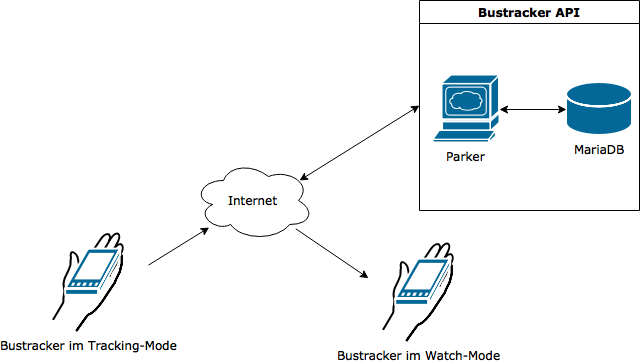
\includegraphics[width=0.8\textwidth]{images/CSArchitektur.png} 
	\caption{Äußere Architektur von \emph{Bustracker}}
	\label{fig:CSArchitektur}
\end{figure}

Die Architektur der App \emph{Bustracker} selbst ist in Abbildung \ref{fig:innereArchitektur} dargestellt. Die App ist eine \glqq Single Page Application\grqq{}. Der interaktive Teil ist als \gls{gls:html}-Komponente mittels <ion-app> - Tag eingebunden. An dieser Stelle wird das \glqq Root-Element\grqq der Komponente geladen. Die Komponente besteht aus \emph{Declarations}, also den Seiten und den \emph{Providers}, diese enthalten die Programmlogik.

\begin{figure}[htbp] 
	\centering
	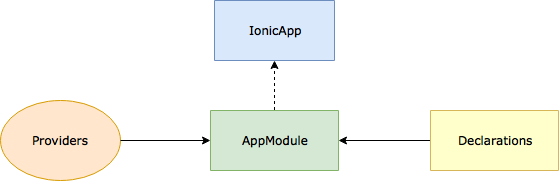
\includegraphics[width=0.8\textwidth]{images/AppArchitektur.png} 
	\caption{Innere Architektur von \emph{Bustracker}}
	\label{fig:innereArchitektur}
\end{figure}

Um \emph{Bustracker} auf verschiedenen Platformen einsetzen zu können, muss es vermieden werden, native Funktionen bestimmter Geräte oder Betriebsysteme direkt zu verwenden. Für diesen Prototypen wurde \nameref{sec:Angular}, ein Framework zur Erstellung von Single Page Applications, eingesetzt. Um die nativen Gerätefunktionen, wie z. B. \gls{gls:gps} oder Bluetooth in \emph{Bustracker} zu nutzen wird \nameref{sec:Cordova} verwendet. 
Bei der Entwicklung kommt \nameref{ionic} als übergeordnetes Framework zum Einsatz. Ionic verwendet verschiedene Befehle und Konzepte von Angular und Cordova bereits implizit. 
Die Entwicklungssprache ist \nameref{typescript}, eine Spracherweiterung von Javascript, mit zusätzlicher Syntax und einer Typisierung.
 

\section{Ionic 4}
\label{ionic}
Die Auswahl des Frameworks begründet sich auf die Antworten folgender Fragen:
\begin{description}
\item[In welchen Sprachen ist der/die Entwickler erfahren?] \hfill \\
Der Entwickler hat Erfahrung in Java und TypeScript. 

\item[Ist es eine native Anwendung oder ist sie webbasiert?] \hfill \\
Die Anwendung soll platformübergreifend funktionieren und die nativen Funktionen des jeweiligen Endgeräts unterstützen. Die Anwendung ist grundsätzlich webbasiert, jedoch ist dies für den Nutzer nicht offensichtlich.

\item[Welche Funktionalitäten werden benötigt und sind diese abgedeckt?] \hfill \\
Die benötigten Funktionen sind \gls{gls:gps}, Bluetooth, iBeacon, Festspeicher und \newline HTTP"~Kommunikation (\gls{gls:http}). Die Funktionen sind über die \emph{native Plugins} abgedeckt.

\item[Werden GUI-Elemente geboten?] \hfill \\
Ionic bietet eine Vielzahl von GUI-Elementen für iOS und Material Design. Diese umfassen vor Allem Interaktions- und Anzeigeelemente. \cite{ionicGUI}

\item[Sind Schnittstellen zu z. B. Datenbanken vorhanden ?] \hfill \\
Verschiedene Schnittstellen können via Plugin nachinstalliert werden.

\item[Ist das Framework zukunftsfähig?] \hfill \\
Ja, das Ionic-Framework wird kontinuierlich weiterentwickelt. Dies lässt sich hervorragend am sogenannten \glqq Pulse\grqq des \emph{Ionic}-Repositories ablesen. \cite{IonicPulses}

\item[Entstehen Kosten für das Framework?] \hfil \\
Ionic unterliegt der sogenannten MIT-Lizenz \cite{mitlizenz} und darf privat sowie kommerziell kostenlos verwendet werden.
\end{description}


Basierend auf den Antworten, wurde das Ionic-Framework ausgewählt. In einem vorangegangenen Praxisprojekt \cite{PraxBerJoSc} wurde Ionic bereits erfolgreich verwendet.


Ionic 4 ist ein frei verfügbares Open-Source SDK zur Entwicklung von nativen und progressiven Web-Apps.
Der besondere Fokus des Frameworks liegt auf mobilen Endgeräten. So kann eine Anwendung gleichzeitig für iOS-, Android- und Windows Phone Geräte entwickelt werden.
Entwickelt werden die Apps auf Basis von \gls{gls:html} 5, \gls{gls:css} 3, Angular 5 und TypeScript. Um auf den einzelnen Geräten die integrierten Hardwarefunktionen nutzen zu können wird Apache-Cordova verwendet. Ionic-Native, ein TypeScript Wrapper für Cordova Plugins wird verwendet, um native Funktionen einfach in die Applikation einzubinden.

Das Ionic Framework steht unter der MIT-Lizenz \cite{mitlizenz}, wodurch es sowohl privat als auch geschäftlich kostenlos verwendet werden kann.

\section{Angular 5}
\label{sec:Angular}
Angular ist ein Web-Framework zur Erstellung von Single-Page Applications (SPA). Es basiert auf TypeScript. Angular verwendet das MVVM-Pattern (Model-View ViewModel). 
Die Komponente (Component) entspricht hier dem ViewModel, welches die UI-Logik enthält. Sie tauscht Daten mit dem Model aus und stellt Methoden und Dienste bereit. 
Die View wird durch Databinding an das ViewModel gebunden und ist somit einfach austauschbar. 
Sie wird unter Verwendung von \gls{gls:html} 5 und \gls{gls:css} 3 erzeugt. 
Das Model enthält alle Inhalte, die durch den Benutzer angezeigt und verändert werden können.
Angular ist seit November 2017 in der Version 5 erhältlich. Das Framework ist Open-Source und Google ist an der Entwicklung beteiligt. Unit-Tests und End-to-End Tests werden von Angular unterstützt.  \cite{angulario}
 

\section{TypeScript}
\label{typescript}
TypeScript ist eine freie Open-Source Programmiersprache, die von Microsoft entwickelt
wird \cite{TSDoc}.  Bei der Programmiersprache handelt es sich um eine typisierte Obermenge von JavaScript.
Sie basiert auf den \gls{gls:ecma} 6 Standard und erweitert die JavaScript Sprache mit einer statischen Typisierung, wie in der Abbildung \ref{img:typescript} zu sehen ist. Um die Kompatibilität zu gewährleisten, ist JavaScript Code gültiger Typescript Code. Ein Browser muss mindestens \gls{gls:ecma} 5 Fähigkeiten haben, damit Typescript ausführbar ist. 
\begin{figure}[htbp]
	\centering
	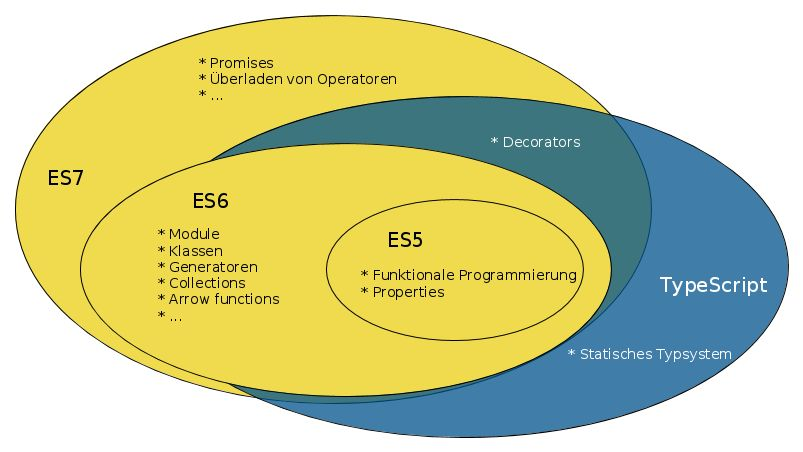
\includegraphics[scale=0.5]{TypeScript.jpg}
	\caption{TypeScript Sprach-Hierachie \cite{tshirachie}}
	\label{img:typescript}
\end{figure} 

%\begin{figure}[htbp] 
 % \centering
 %    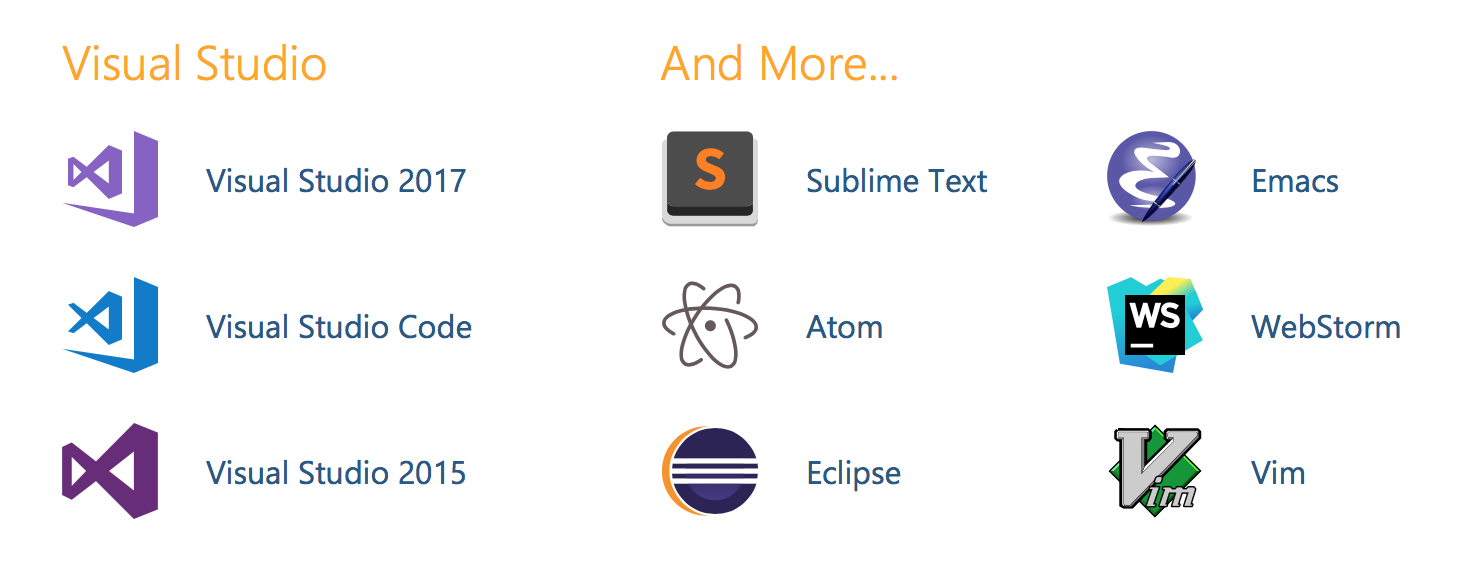
\includegraphics[width=0.8\textwidth]{images/idestypescript.png} 
%  \caption{Empfohlene IDEs für TypeScript}
 % \label{fig:IDEs}
% \end{figure}

\section{Cordova}
\label{sec:Cordova}
Apache Cordova ist ein Open Source Framework zur Entwicklung für mobile Plattformen. Mit Cordova ist es möglich moderne Web-Technologien, wie \gls{gls:html} 5, \gls{gls:css} 3 und JavaScript (hier TypeScript) für plattformübergreifende Entwicklung zu nutzen. Um auf die Sensoren und Daten der einzelnen Geräte zuzugreifen werden Standard APIs der einzelnen Betriebssysteme verwendet. Cordova dient als Mittelschicht zwischen Anwendung und Gerät \cite{cordovaDoku}. Abbildung \ref{img:cordova} zeigt den allgemeinen Aufbau der Architektur.
\begin{figure}[htbp]
	\centering
	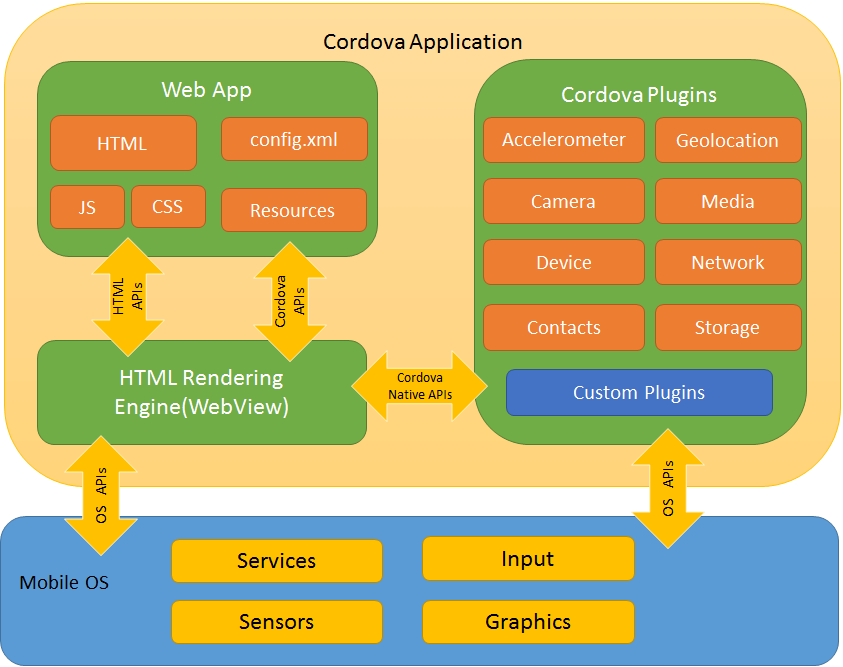
\includegraphics[width=0.6\textwidth]{cordova.png}
	\caption{Architektur von Cordova \cite{cordovaDoku}}
	\label{img:cordova}
\end{figure}

\section{iBeacon}
Sogenannte iBeacons sind Bluetooth Low Energy Sender, die nach einem proprietärem von Apple spezifizierten Protokoll, dem iBeacon Protokoll \cite{iBeaconSpec}, arbeiten. Die Idee hinter der Entwicklung der iBeacons war die Durchführung von Lokalisation innerhalb von Gebäuden. Beacons eignen sich aber auch für den Gebrauch im Freien, damit können unabhängig des \gls{gls:gps}-Signals Ereignisse, wie das Erreichen oder Verlassen eines bestimmten Bereichs detektiert werden. Abbildung \ref{img:ibeacon} zeigt eine schematische Darstellung der Technologie.
Zur Identifizierung eines einzelnen Beacons werden bei \emph{Bustracker} vier Parameter verwendet, die nachfolgend erläutert werden:

\begin{description}
\item[UUID] \hfill \\
Die \gls{gls:UUID} gibt in diesem Falle die sogenannte Region an. Eine Beacon Region ist keine Region im Sinne von einem durch geografische 
Merkmale begrenztem Bereich. Sie wird durch die Parameter \gls{gls:UUID}, Major und Minor charakterisiert. So wie ein einzelnes Beacon durch die gleichen Parameter gekennzeichnet ist. Die physische Repräsentation einer Beacon Region ist die Reichweite aller dieser Region zugeordneten Beacons. 
Mehrere iBeacons können die gleiche \gls{gls:UUID} haben. 
Alle Beacons mit der gleichen \gls{gls:UUID} gehören zur gleichen Region. \cite{beaconRegion}

Zum Beispiel könnten 100 Beacons mit der gleichen 
\gls{gls:UUID} einem Busunternehmen zugeordnet sein.
\item[Major] \hfill \\
Der Major-Parameter unterteilt die Beacons einer \gls{gls:UUID}. Zum Beispiel könnte dies eine Linie (Strecke) des Busunternehmens sein.
\item[Minor] \hfill \\
Der Minor-Parameter unterteilt eine Major-Gruppe in einzelne Beacons. Dies könnte einer Haltestelle auf einer Linie entsprechen.
\item[Identifier]\hfill \\
Identifier ist ein String um ein Beacon zu beschreiben. Zum Beispiel könnte das hier der Name der Haltestelle sein.
\end{description}

\begin{figure}[htbp]
	\centering
	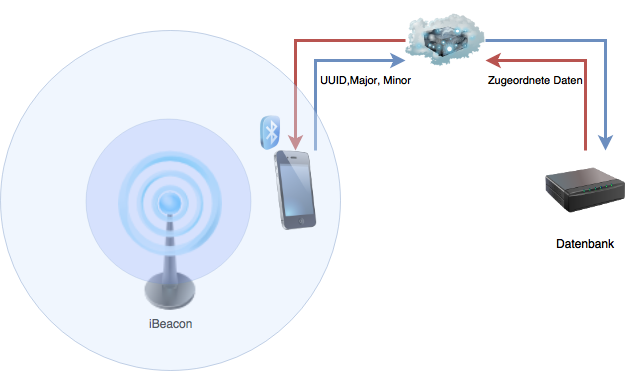
\includegraphics[scale=0.7]{images/iBeacon_schema.png}
	\caption{Schematische Darstellung der iBeacon-Technologie}
	\label{img:ibeacon}
\end{figure} 

Zur konkreten Anwendung kommt diese Technologie im \nameref{srv:iBeaconService}. 

\section{REST}
\label{REST}

\gls{gls:rest} bedeutet Representational State Transfer und beschreibt eine Architektur. Eine \gls{gls:rest} \gls{gls:API} ist \textbf{statuslos}, d. h. es gibt keine Nutzersessions. Jede Anfrage erzeugt eine neue Ressource, alle Daten werden nochmals
generiert. Jede dieser Ressourcen ist über eine spezifische URI adressierbar. Ressourcen können in unterschiedlichen Repräsentationen vorliegen. Die gleiche Information kann in unterschiedlichen Formaten abgerufen werden,
z. B. \gls{gls:html} und \gls{gls:json}. 
\cite{Abts2015}

\section{Werkzeuge}

\subsection{WebStorm}
Aus einem vorhergehenden Projekt war die integrierte Entwicklungsumgebung WebStorm bereits bekannt. 
 
In WebStorm sind die Technologien \gls{gls:html}5, TypeScript, Angular und Cordova bereits integriert. Die \gls{gls:IDE} lässt sich durch ein breites Angebot an Plugins erweitern. Webstorm basiert auf der IntelliJ IDEA Plattform und verwendet Konzepte, die bereits durch \glspl{gls:IDE} wie AndroidStudio bekannt sind. 
WebStorm ist auf JavaScript spezialisiert und bietet darauf zugeschnittene Funktionen wie z. B. Codevervollständigung, automatisches Importieren, Signaturinformationen bei Funktionsaufruf und kontextbezogene Hervorhebung von Syntax. Die Integration von Git/Github erwies sich ebenfalls als sehr hilfreich. Es wird kein weiteres Programm neben der \gls{gls:IDE} benötigt.
Das Interface ist in Abbildung \ref{fig:WebStorm} zu sehen.
 
  \begin{figure}[htbp] 
  \centering
     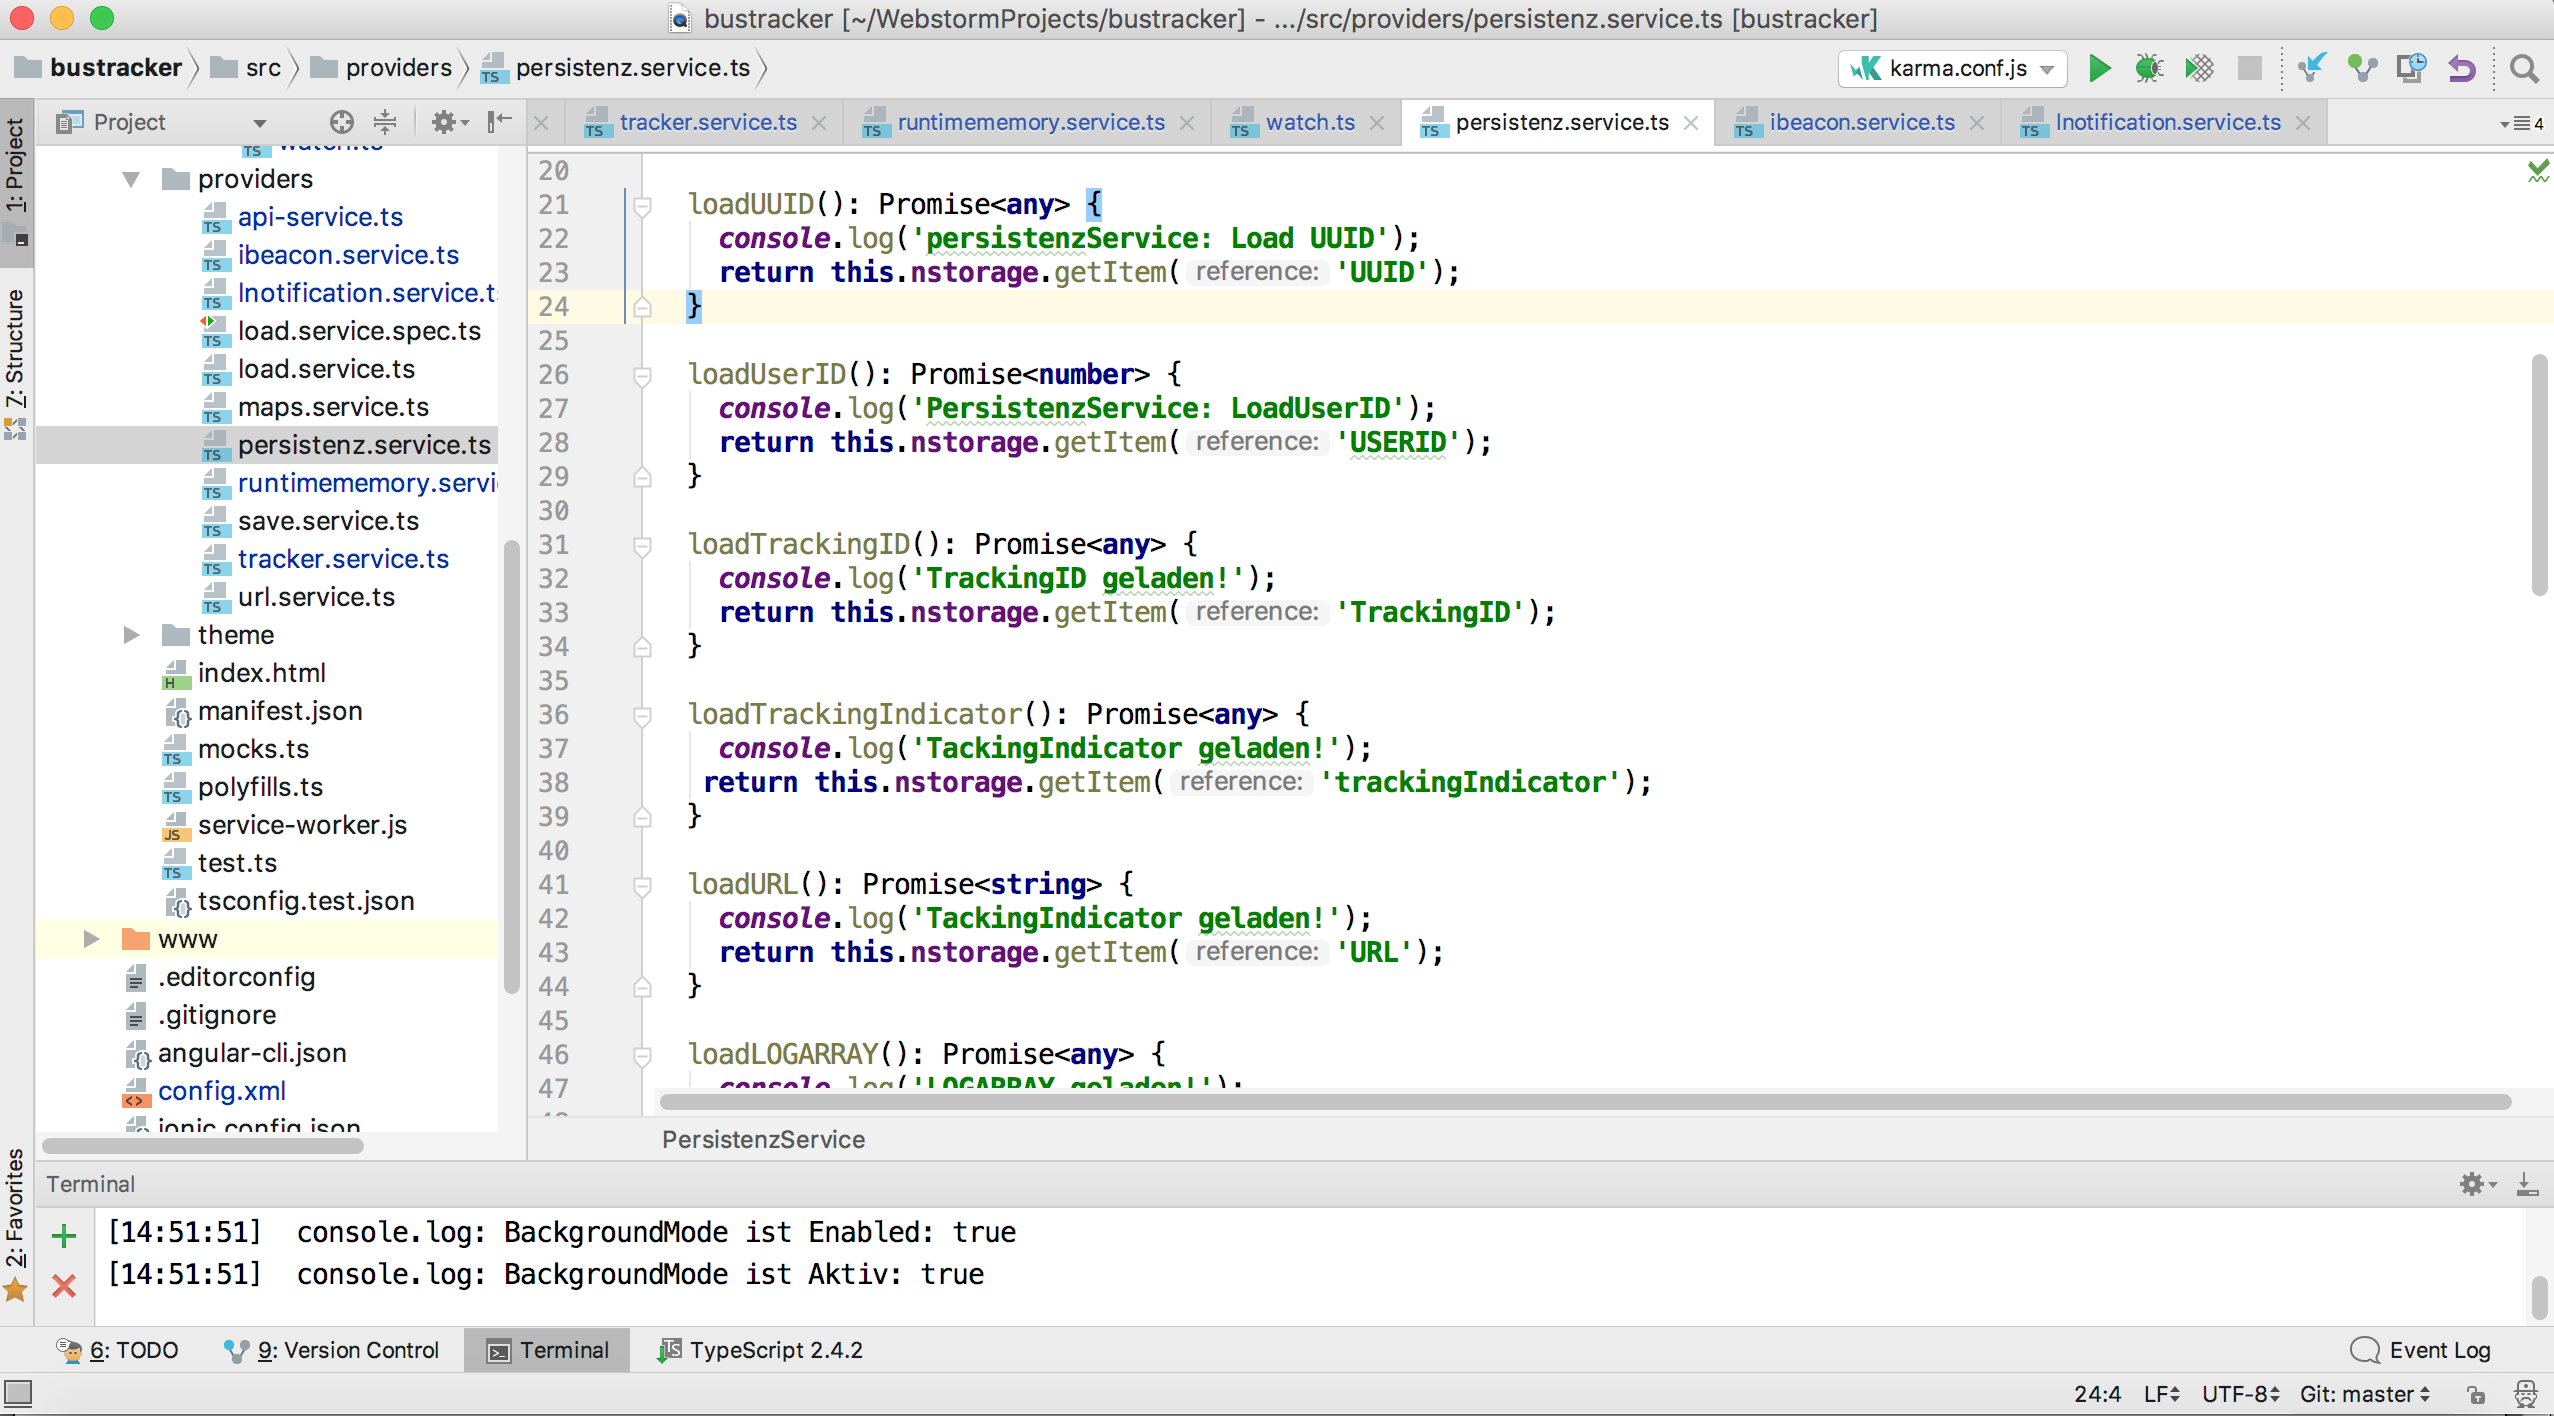
\includegraphics[width=0.9\textwidth]{images/webstorm_weiss.png} 
  \caption{Interface der WebStorm IDE}
  \label{fig:WebStorm}
\end{figure}

\subsection{compodoc}
\label{compodoc}

Um die Verständlichkeit und die Wartbarkeit von Software zu gewährleisten muss eine Dokumentation zum Programmcode existieren. Ein großer Teil der Dokumentation besteht aus Quellcodedokumentation. Der Dokumentationsprozess ist in der Regel aufwendig und bedeutet für die Entwickler zusätzliche Arbeit. Dies führt häufig zu einer lückenhaften und unvollständigen Dokumentation der Software. Um dem vorzubeugen gibt es Tools, die diesen Prozess vereinfachen. 
\textbf{Compodoc} ist ein solches Tool.

Compodoc ist kommandozeilenbasiert und erzeugt eine statische codebasierte Quellcodedokumentation von Angularanwendungen. Die Codedokumentation ist in der Struktur einer Website ausgeführt, sie umfasst eine aufbereitete Ansicht der vom Entwickler im Code eingefügten Kommentare, so dass diese nicht mehrmals geschrieben werden müssen. 
Es besteht die Auswahl zwischen verschiedenen Themes bzw. Templates. Die Templates sind bereits responsiv und unterstützen moderne Webtechnologien.

Diese \glqq Website\grqq{}  wird lokal gehostet und benötigt somit keinen externen Server. Eine mächtige Such-Engine namens \glqq lunr.js\grqq{} sorgt dafür, dass die Dokumentation effizient durchsucht werden kann. Compodoc parsed den Code lediglich, es ist keine TypeScript-Kompilierung notwendig. Durch das Parsen enthält die Dokumentation alle Elemente der Anwendung automatisch. Sie sind im Inhaltsverzeichnis gelistet. Es besteht die Möglichkeit zu jeder Komponente den Quellcode direkt einzusehen. Kommentare die im JSDoc-Format \cite{JSdoc} vorliegen, werden von Compodoc \glqq verstanden\grqq{} und in die Codedokumentation mit aufgenommen. Zur Zeit kann Compodoc \glqq @param, @returns, @link und @example\grqq verarbeiten. Abbildung \ref{fig:JSDemo} zeigt den Quellcode und das Compodoc Ergebnis.

\begin{figure}[htbp] 
	\centering
	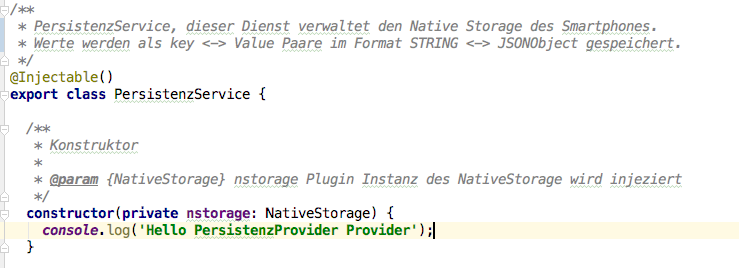
\includegraphics[width=0.9\textwidth]{images/composource.png} 
	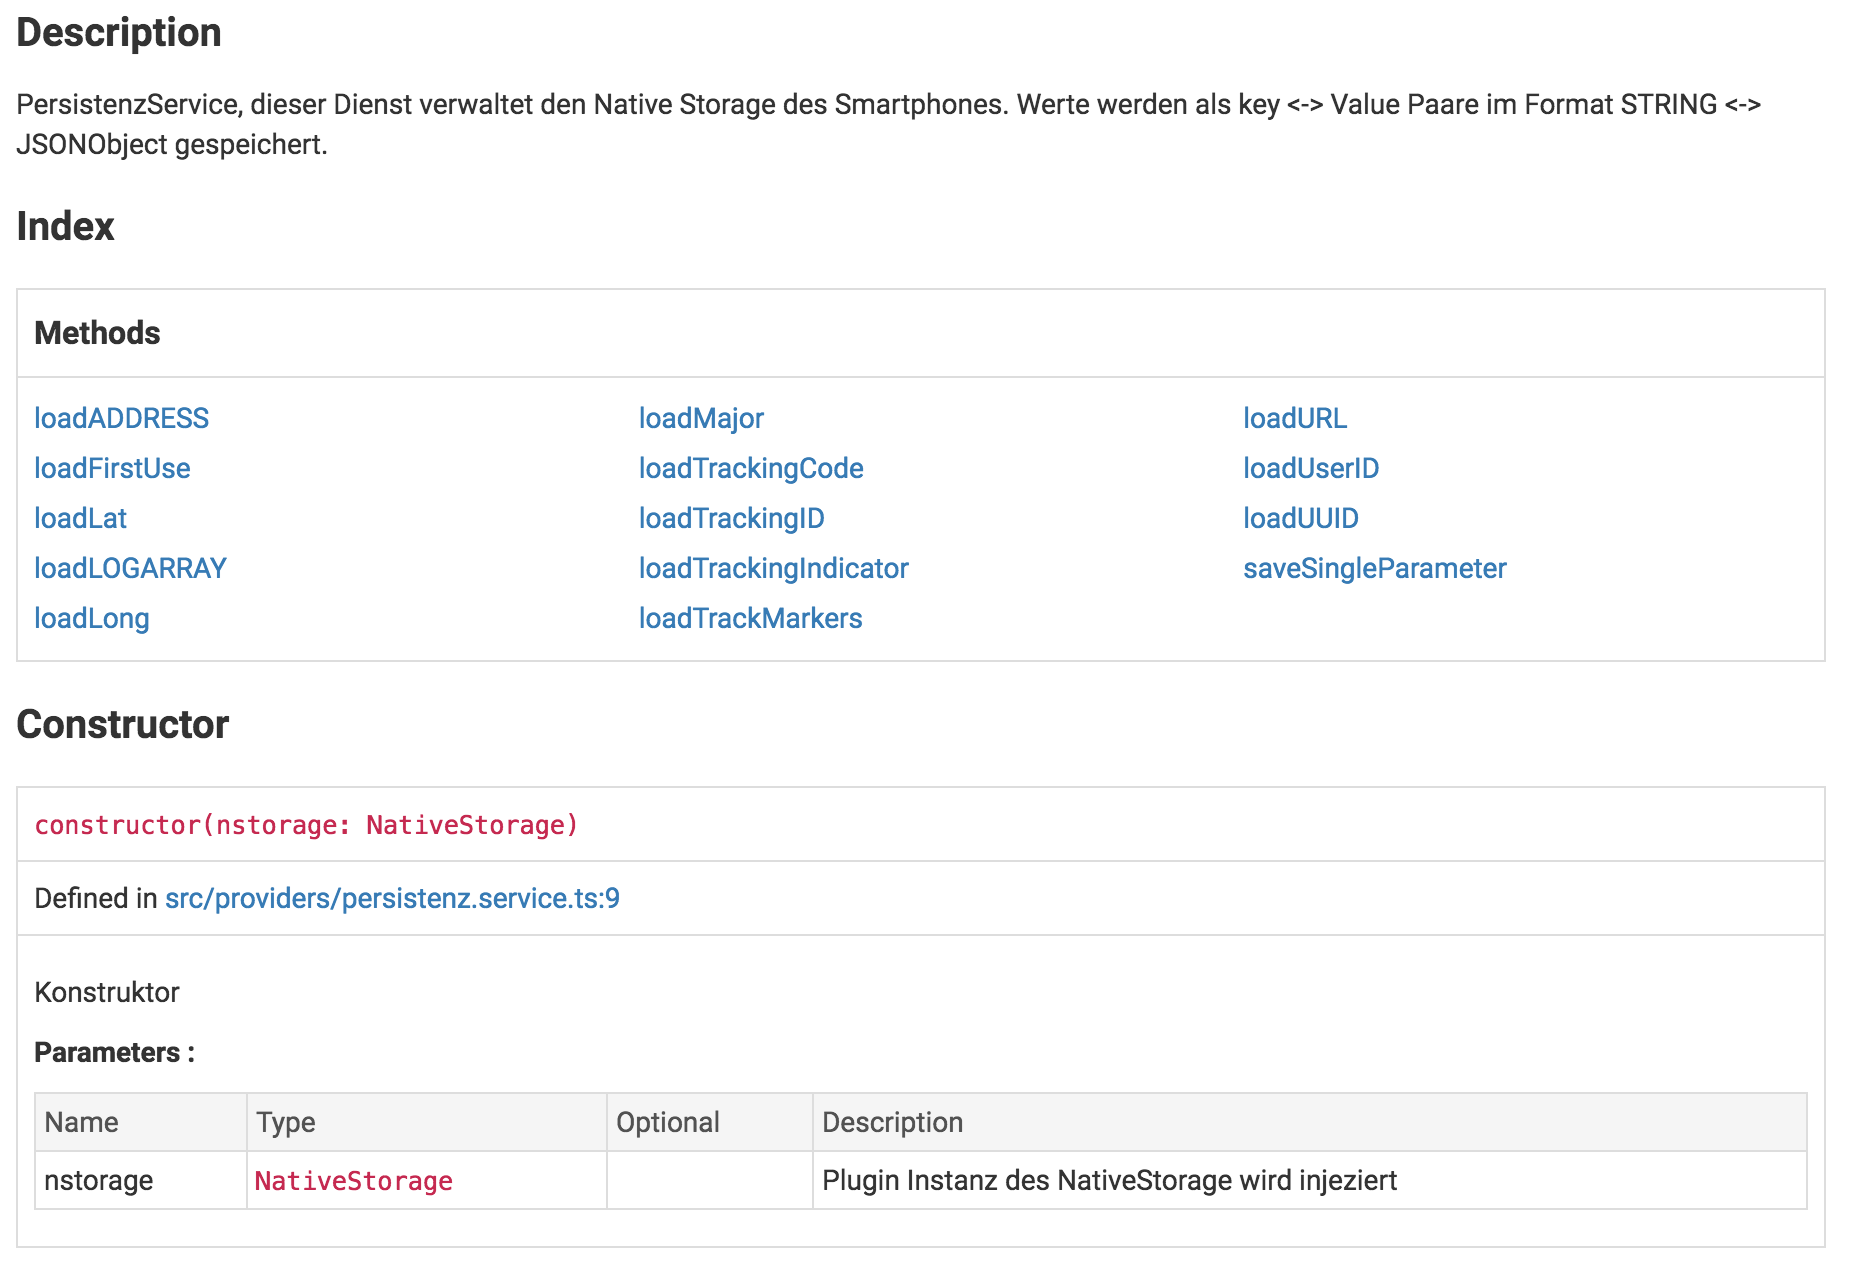
\includegraphics[width=0.9\textwidth]{images/compoergebnis.png}
	\caption{TypeScript Quellcode und Compodoc Seite im Vergleich.}
	\label{fig:JSDemo}
\end{figure}

	% !TeX root = Bachelorarbeit.tex
\chapter{Organisation}
\label{Organisation}
\section{Workflow}
Der bereits im Praxisprojekt \cite{PraxBerJoSc} etablierte Workflow wurde zu einem großen Teil übernommen. 
Tägliche Treffen jedoch entfielen, da der Autor nicht in einem Team arbeitete.

Anforderungen an die Software wurden als Stories in dem \glqq Issues \grqq-Tab des verwendeten GitHub Repositories als User Story eingetragen. Abbildung  \ref{fig:EinzelStory} zeigt eine solche Story.


\begin{figure}[htbp] 
  \centering
     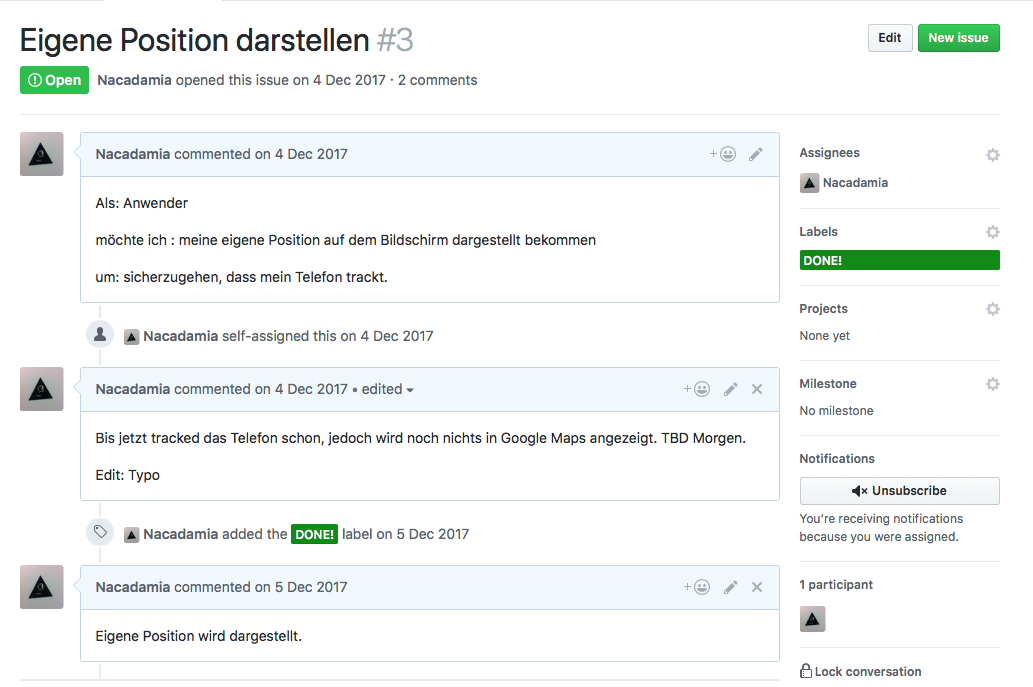
\includegraphics[width=0.8\textwidth]{images/EinzelStory.png} 
  \caption{Einzelne Story im Issues-Tab des \emph{Bustracker} Repository}
  \label{fig:EinzelStory}
\end{figure}

Es wurden Stories aus dem in Abbildung \ref{fig:IssuesTab} gezeigten IssusesTab gewählt. Nach Abschluss einer Story bzw. Implementierung eines Features, wurde diese mit dem Label \glqq Done\grqq{} versehen. Nach positiver Abnahme wurde die Story dann auf \glqq closed\grqq{} gesetzt und somit geschlossen.

\begin{figure}[htbp] 
  \centering
     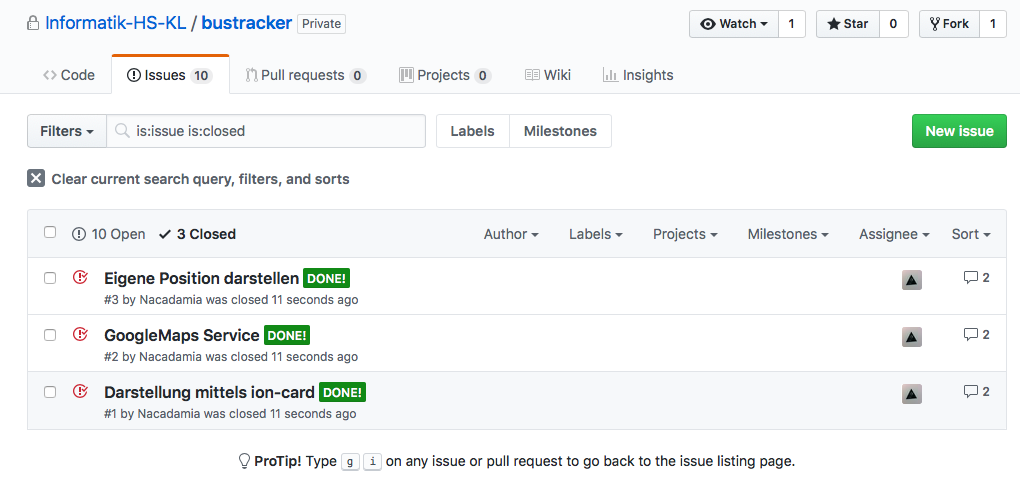
\includegraphics[width=0.8\textwidth]{images/issues_tab.png} 
  \caption{Issues-Tab des Repository}
  \label{fig:IssuesTab}
\end{figure}

Um die Positionsdaten zu erfassen und im Anschluß wieder zu verteilen wird eine Datenbank benötigt. Die gewählte Datenbank ist eine sogenannte MariaDB \cite{MariaDBDoku}.
Die gewählte Datenbankstruktur und die benötigten Daten sind in Abb. \ref{fig:ERD} dargestellt.

\begin{figure}[htbp] 
	\centering
	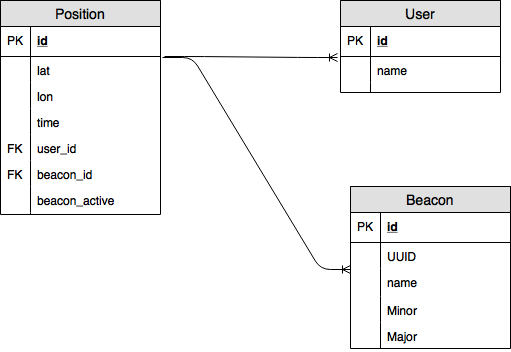
\includegraphics[width=0.8\textwidth]{images/ERDiagramm_bustracker.png} 
	\caption{ER-Diagramm der Bustracker Datenbank}
	\label{fig:ERD}
\end{figure}

 Die API-Entwicklung wurde extern durchgeführt. Die entstandene REST-API ist in \cite{btapidoku} beschrieben. 
\section{Ablauf}

Zu Beginn der Arbeit wurden die benötigten Funktionalitäten für \emph{Bustracker} identifiziert. Diese wären zum einen die Möglichkeiten zur Positionsbestimmung \gls{gls:css} und iBeacons und zum anderen die Anzeige der zuvor bestimmten Position. Dies wurde mittels der Brainstorming Technik durchgeführt. (Abbildung \ref{fig:Brainstorming}).

Für den Prototypen kommt hier aufgrund der einfachen Implementierung und umfangreicher \glspl{gls:API}  GoogleMaps in Frage. Um den Zustand der App speichern zu können bot sich der Zugriff auf den Festspeicher des jeweiligen Endgerätes an.  Um dem eigentlichen Zweck, die Mitteilung der eigenen Position an ein anderes Endgerät zu übertragen, zu entsprechen, müssen die Daten weitergeleitet werden.  Dazu wird bei \emph{Bustracker} eine \nameref{REST} - \nameref{API} eingesetzt.  

\begin{figure}[htbp] 
  \centering
     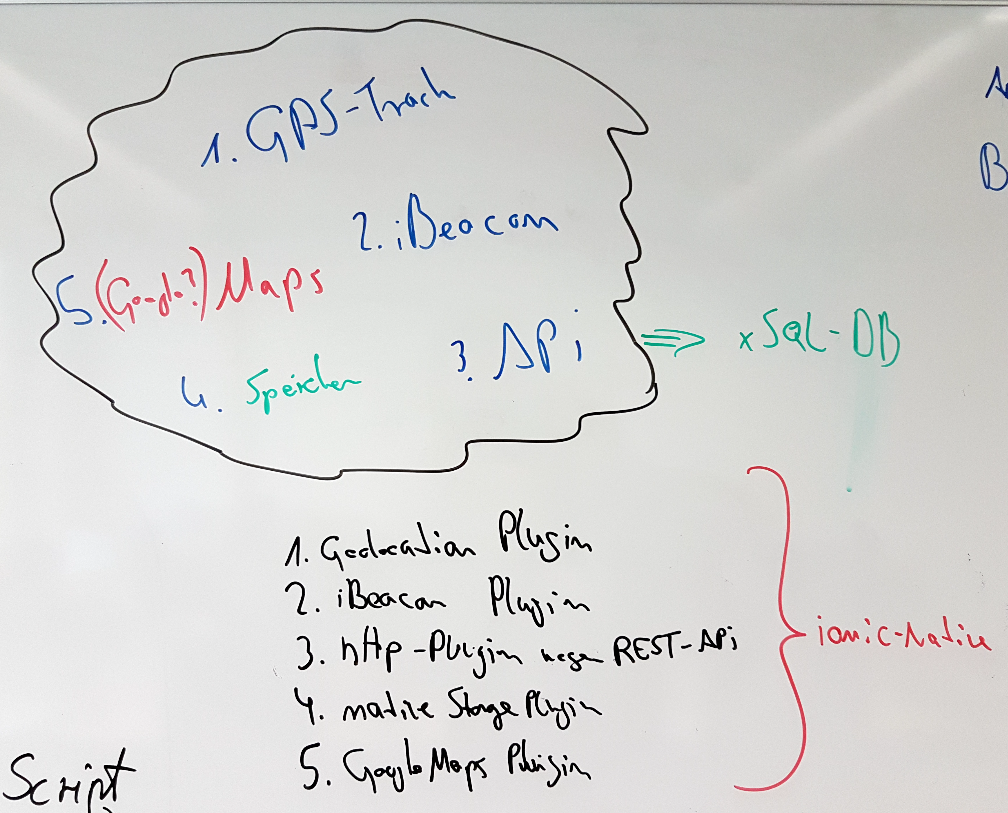
\includegraphics[width=0.8\textwidth]{images/brainstorming.png} 
  \caption{Ergebnis des Brainstormings}
  \label{fig:Brainstorming}
\end{figure}

\nameref{ionic} bietet eine Reihe von Plugins an, mit denen die native Hardware des Gerätes plattformunabhängig angesprochen wird. Alle Funktionen können mittels solcher \emph{native Plugins} abgebildet werden. Zur konkreten Implementierung siehe Kapitel \nameref{Backend}.

Im Anschluss an diesen Teil erfolgte die Implementierung von Teilfunktionen um mehr über das Verhalten der einzelnen Plugins herauszufinden. Parallel wurde das Aussehen des \gls{gls:gui} in sogenannten Scribbles skizziert. Ein Beispiel ist das Scribble der WatchPage in Abbildung \ref{fig:scribble}. 

\begin{figure}[htbp] 
  \centering
     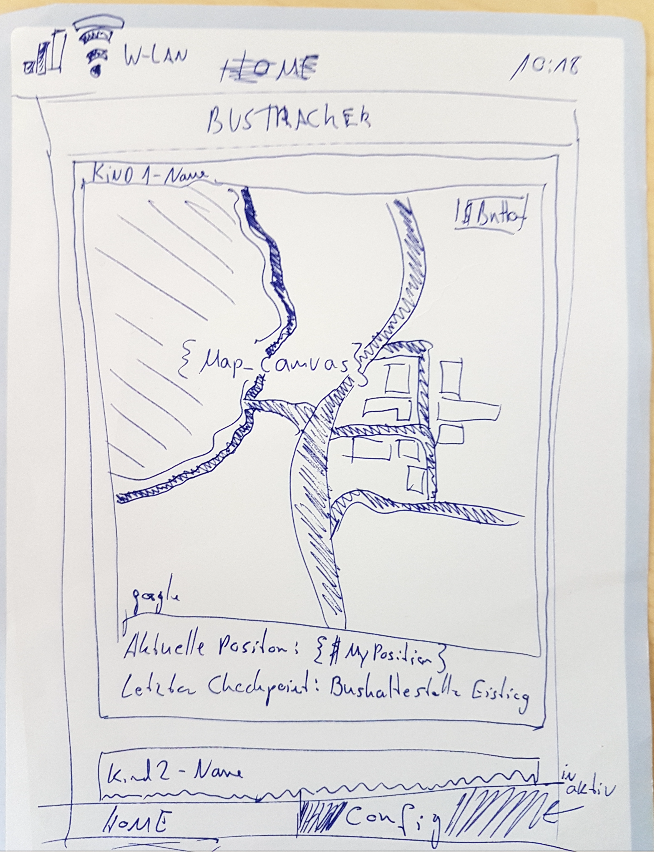
\includegraphics[width=0.6\textwidth]{images/scribble.png} 
  \caption{Scribble der WatchPage}
  \label{fig:scribble}
\end{figure}

Nach dem Vorbild der Scribbles wurden die Seiten gestaltet. Im Anschluss daran wurden die Komponenten ausgewählt, um die geplanten Funktionalitäten bereitzustellen. Diese Komponenten wurden eingebunden und damit der gewünschte Funktionsumfang geschaffen. Nachdem die Komponenten erfolgreich getestet wurden, erfolgte die externe Anbindung an die \gls{gls:API}.
Am Ende wurde die Benutzeroberfläche einheitlich gestaltet.


	
	
	%\input{anhang}
	
	\singlespacing

	\bibliography{literatur}
	\bibliographystyle{apalike}
	\nocite{*} % nicht referenzierte Literatur anzeigen
	\addcontentsline{toc}{chapter}{Literatur}
	
	%\newpage
	
	%\printglossary[title=Abkürzungsverzeichnis, type=\acronymtype, style=long]




%\begin{appendix}
	
	%\chapter{Anhang}	
	
%\end{appendix}
	
	

\raggedright

%\todos

\end{document}
